\documentclass{beamer}

%\usetheme{Boadilla}
\usetheme{Frankfurt}
%\usetheme{Ilmenau}
%\usetheme{Madrid}
%\usetheme{PaloAlto}

\usepackage{graphicx}
\usepackage{color}

\title{First Order Optimization Methods in Training Deep Neural Networks}
% \subtitle{Optional Subtitle}

\author{Rui Zhang \and Yujia Liu}

\date{April 2015}

\subject{}
% This is only inserted into the PDF information catalog. Can be left
% out.

\pgfdeclareimage[height=0.5cm]{university-logo}{gatech}
\logo{\pgfuseimage{university-logo}}

% Let's get started
\begin{document}

\begin{frame}
  \titlepage
\end{frame}

\begin{frame}{Outline}
  \tableofcontents
  % You might wish to add the option [pausesections]
\end{frame}

\section{Objective}

\begin{frame}{Objective}
    
\begin{itemize}
    \item Framework
    \\
    Build a Stacked Denoising Autoencoder to classify datasets such as MNIST and CIFAR.
    \item Algorithms
    \\
    Implement different First Order Optimization algorithms and compare them in terms of accuracy, converge rate, etc.
\end{itemize}

\end{frame}


\section{Datasets}

\subsection{MNIST}
\begin{frame}{MNIST}
The MNIST database of handwritten digits has a training set of 60,000 examples, and a test set of 10,000 examples. The digits have been size-normalized and centered in a 28x28 fixed-size image. 

\begin{figure}[h!]
\centering
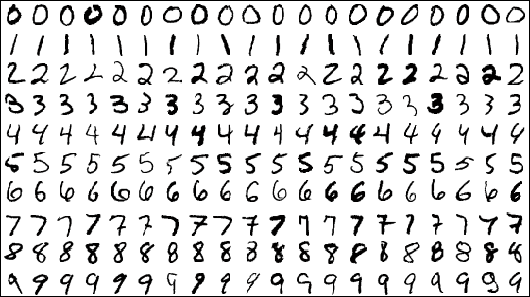
\includegraphics[width=0.4\textwidth]{MNIST.png}
\end{figure}

\begin{thebibliography}{9}
\beamertemplatebookbibitems
\bibitem{MNIST}
LeCun Y, Bottou L, Bengio Y, et al.
\newblock {\em Gradient-based learning applied to document recognition}.
\end{thebibliography}

\end{frame}

\subsection{CIFAR}
\begin{frame}{CIFAR}
The CIFAR-10 dataset consists of 60000 32x32 colour images in 10 classes, with 6000 images per class. There are 50000 training images and 10000 test images.
    
\begin{figure}[h!]
\centering
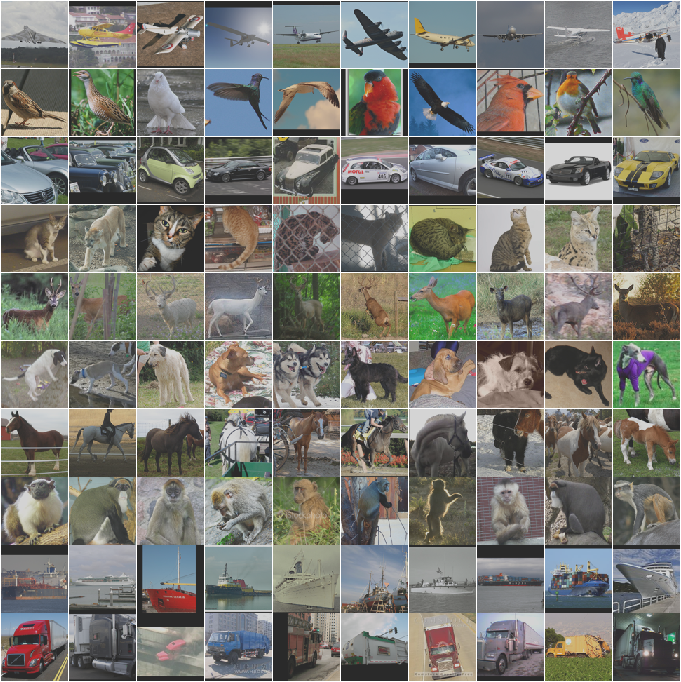
\includegraphics[width=0.4\textwidth]{CIFAR-10.png}
\end{figure}

\begin{thebibliography}{9}
\beamertemplatebookbibitems
\bibitem{CIFAR}
Krizhevsky A, Hinton G
\newblock {\em Learning multiple layers of features from tiny images}.
\end{thebibliography}

\end{frame}


\section{Framework}

\subsection{Denoising Autoencoder}
\begin{frame}{Denoising Autoencoder}
A denoising autoencoder neural network is an unsupervised learning algorithm that stochastically corrupts the signal. This architecture attempts to capture the representation of the signal that is invariant to noise.

\begin{figure}[h!]
\centering
\includegraphics[width=0.7\textwidth]{denosing.png}
\end{figure}

\end{frame}

\subsection{Softmax}
\begin{frame}{Softmax}
Softmax model generalizes logistic regression to classification problems where the class label can take on more than two possible values. 
%This will be useful for such problems as MNIST digit classification, where the goal is to distinguish between 10 different numerical digits.

\begin{equation*}
h_{\theta}(x^{(i)})=
\left[\begin{array}{cccc}
P(y^{(i)}=1|x^{(i);\theta})\\
P(y^{(i)}=2|x^{(i);\theta})\\
\vdots\\
P(y^{(i)}=k|x^{(i);\theta})\\
\end{array}\right]
=\frac{1}{\sum^k_{j=1}e^{\theta^T_j x^{(i)}}}
\left[\begin{array}{cccc}
e^{\theta_1^T x^{(i)}}\\
e^{\theta_2^T x^{(i)}}\\
\vdots\\
e^{\theta_k^T x^{(i)}}\\
\end{array}\right]
\end{equation*}



\end{frame}

\subsection{Stacked Denoising Autoencoders}

\begin{frame}{Stacked Denoising Autoencoders}
A stacked denoting autoencoder is a neural network consisting of multiple layers of denoising autoencoders in which the outputs of each layer is wired to the inputs of the successive layer.

%you would feed the primary features into the second sparse autoencoder to obtain the secondary feature activations for each of the primary features (which correspond to the primary features of the corresponding inputs). You would then treat these secondary features as "raw input" to a softmax classifier, training it to map secondary features to digit labels.

\begin{figure}[h!]
\centering
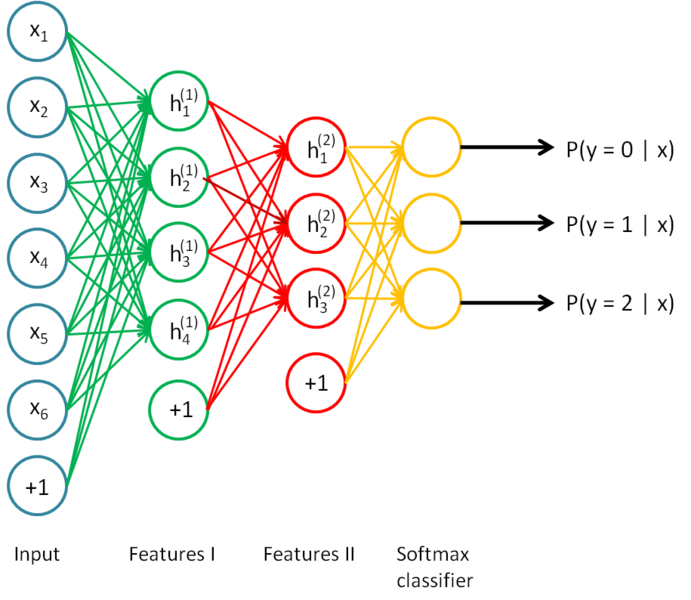
\includegraphics[width=0.6\textwidth]{Stacked.png}
\end{figure}

\end{frame}

\section{Algorithms}

\subsection{First Order Algorithm}
\begin{frame}{Methods we implemented}
\begin{itemize}
\item Stochastic Gradient Descent 
\item Adaptive Gradient Descent
\item Nesterov's  Accelerated Gradient
\end{itemize}

\begin{thebibliography}{9}
\beamertemplatebookbibitems
\bibitem{CIFAR}
John Duchi 
\newblock {\em Adaptive Subgradient Methods for
Online Learning and Stochastic Optimization}.
\end{thebibliography}

\begin{thebibliography}{9}
\beamertemplatebookbibitems
\bibitem{CIFAR}
Ilya Sutskever
\newblock {\em On the importance of initialization and momentum in deep learning}.
\end{thebibliography}


\end{frame}


\begin{frame}{Why First Order}
Reasons not to choose second order optimization methods like L-BFGS 
\begin{itemize}
\item Constructing a Hessian Matrix is memory consuming
\begin{itemize}
\item $28*28$ image, $100$ hidden units a layer, single layer, double precision: $(28*28*100*1)^2= 0.331776e9 \text{ byte }=0.3GB$, Somewhat acceptable 
\item $256*256$ image,... : $6978*0.3GB$ =Unacceptable 
\end{itemize}
\item Computational expensive and no clear improvements for highly non convex neural networks compared to First Order Methods
\end{itemize}
\end{frame}

\begin{frame}{Minibatch Optimization}
Suppose Dataset is $D$ and the loss function is defined as 
$$
L(w)=\frac{1}{D}\sum_i^D F_w(x_i)+\lambda R(w)
$$
Instead of using all the dataset( batch) or randomly picked one( sequential), use a small set of the training data to find the gradients and update.
$$
L(w)\approx \frac{1}{N} \sum_i^N F_w(x_i)+\lambda R(w)
$$
\end{frame}


\subsection{Methods Details}
\begin{frame}{Optimization in a long narrow Valley}
\begin{itemize}
\item Highly non-convex loss function
\item Loss function is the Long narrow valley and the arrow is the gradient descent direction
\end{itemize}
\begin{figure}[h!]
\centering
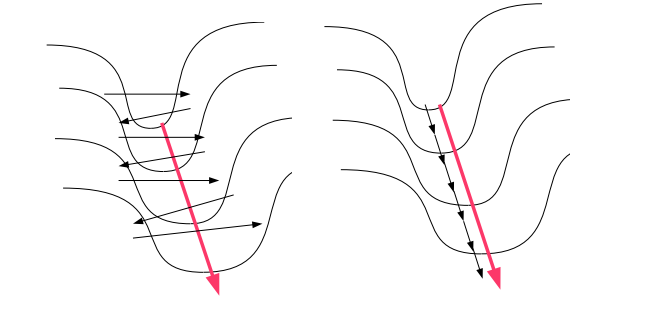
\includegraphics[width=0.6\textwidth]{narrow.png}
\end{figure}

\end{frame}




\begin{frame}{SGD}

Suppose momentum, the weight of previous update is $\mu$, the learning is $\alpha$, the Weights $W$ are updated in the following fashion
$$
V_{t+1}=\mu V_t-\alpha \triangledown L(W_t)
$$
$$
W_{t+1}=W_t+V_{t+1}
$$
Rules of setting $\alpha$ and $\mu$
\begin{itemize}
\item $\mu=0.5$ in the beginning and set to $0.9$ later 
\item $\alpha$=0.01 is a good start and drop by 10 when loss reaches a plateau
\end{itemize}
\end{frame}

\begin{frame}{AdaGrad}
\begin{itemize}
 \item Per-feature learning rate $ \alpha_{t,i}=\frac{\alpha}{\sqrt{G_{ti}}}=\frac{\alpha}{\sqrt{\sum_1^t W_{t',i}^2}} $
 \item Update Rule $W_{t+1,i}=W_{t,i}-\frac{\alpha}{\sqrt{\sum_1^t W_{t',i}^2}} \triangledown L(W_t)$
 \end{itemize}
 Implementations details: Only O(f) extra storage and one extra element wise vector multiplication is needed.\\
 Advantage: Sparse features are weighted more and thus could help higher recognition rate.
\end{frame}

\begin{frame}{NAG}
Compared to SGD, weights are also updated when computing the loss function.
$$
V_{t+1}=\mu V_t-\alpha \triangledown L(W_t+\mu V_t)
$$
$$
W_{t+1}=W_t+V_{t+1}
$$
Advantage: If $\mu V_t$ is a poor update, then $\triangledown L(W_t+\mu V_t)$ will point backwards to $W_t$ more than $\triangledown L(W_t)$
\end{frame}

\section{Experiment \& Result}
\begin{frame}{Convergence Plot of MNIST}
\begin{figure}[h!]
\centering
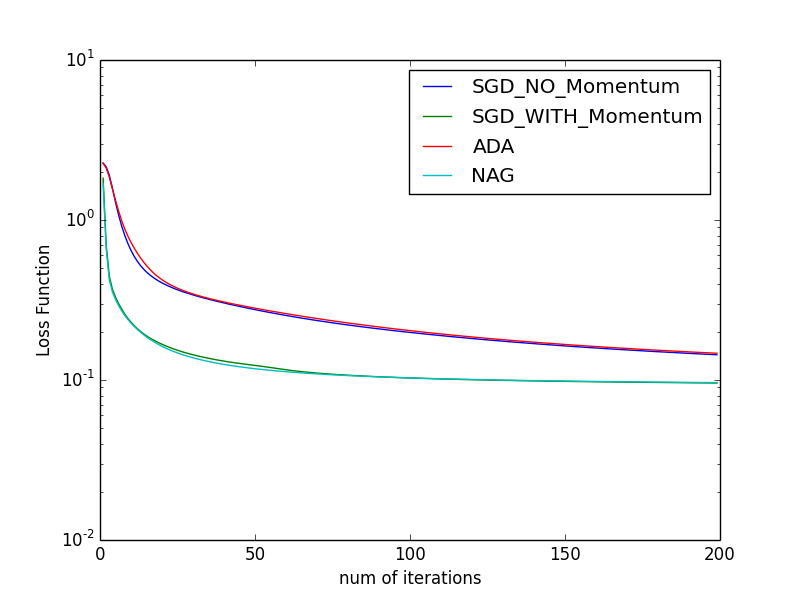
\includegraphics[width=0.6\textwidth]{Mnist_Convergence.png}
\caption{Convergence Rate of different algorithms}
\end{figure}
NAG and SGD(Momentum) seems to drop faster than the other two.
\end{frame}


\begin{frame}{Test Error of MNIST}
After 200 iterations, the corresponding test error is 
\begin{table}[h]
\begin{tabular}{|l|l|l|l|l|}
\hline
      & SGD(No Momentum) & SGD    & ADA    & NAG    \\ \hline
Error & 3.22\%           & \textbf{1.82\%} & 3.28\% & 2.16\% \\ \hline
\end{tabular}
\caption{Error}
\label{my-label}
\end{table}


\begin{table}[h]
\begin{tabular}{|l|l|l|l|l|}
\hline
             & SGD(No Momentum) & SGD    & ADA  & NAG  \\ \hline
Time(minutes) & 9.1973           & \textbf{8.9759} & 9.94 & 9.15 \\ \hline
\end{tabular}
\caption{Running time}
\label{my-label}
\end{table}

SGD with momentum outperforms other methods in both recognition rate and running time.
\end{frame}



\begin{frame}{Convergence Plot of Cifar10}
\begin{figure}[h!]
\centering
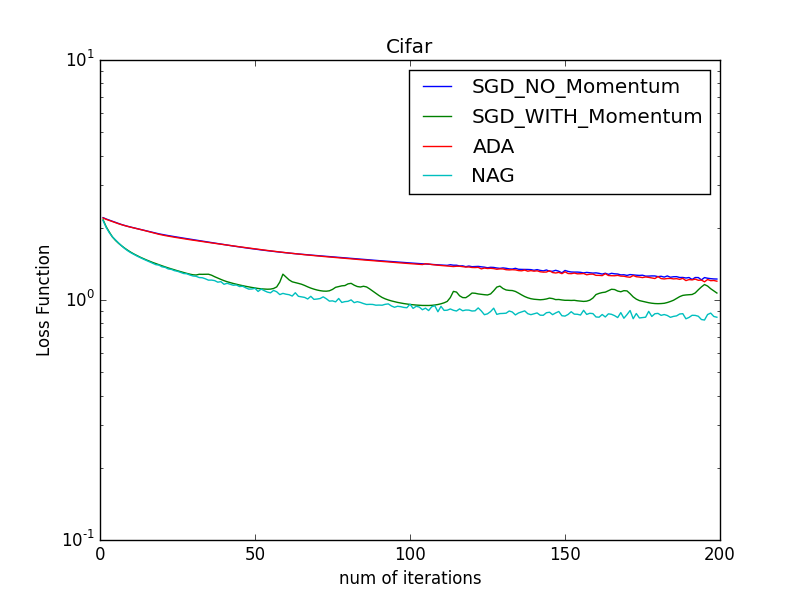
\includegraphics[width=0.6\textwidth]{Cifar_Convergence.png}
\caption{Convergence Rate of different algorithms}
\end{figure}
NAG and SGD(Momentum) still outperforms the other two. But SGD is more volatile.
\end{frame}



\begin{frame}{Test Error of Cifar}
With 100 hidden units and 200 iterations, the corresponding test error is 
\begin{table}[h]
\begin{tabular}{|l|l|l|l|l|}
\hline
      & SGD(No Momentum) & SGD    & ADA    & NAG    \\ \hline
Error & 53.22\%           & 51.82\% & \textbf{47.28\%} & 52.16\% \\ \hline
\end{tabular}
\caption{Error}
\label{my-label}
\end{table}


\begin{table}[h]
\begin{tabular}{|l|l|l|l|l|}
\hline
             & SGD(No Momentum) & SGD    & ADA  & NAG  \\ \hline
Time(minutes) & 26.79           & \textbf{27.09} & 29.78 & 28.12 \\ \hline
\end{tabular}
\caption{Running time}
\label{my-label}
\end{table}
This time ADA performs best but more number of hidden units are called for to increase the capacity of the model. 

\end{frame}






\begin{frame}{Sensitivity to Learning Rate}
\begin{table}[h]
\begin{tabular}{|l|l|l|l|l|}
\hline
            & SGD(no Momentum) & SGD     & Ada     & NAG     \\\hline
$\alpha$=1    & \color{red}2.26\%           & 70.02\% & 45.09\% & 43.12\% \\\hline
$\alpha$=2e-1 & 2.12\%           &\color{red} 1.98\%  & 2.12\%  & 2.23\%  \\\hline
$\alpha$=2e-2 & 7.57\%           & 2.78\%  & \color{red} 2.34\%  & 3.12\%  \\\hline
$\alpha$=2e-3 & 18.09\%          & 7.12\%  &\color{red}  6.78\%  & 7.45\%  \\\hline
$\alpha$=2e-4 & 59.23\%          & 19.12\% & \color{red} 13.63\% &   21.12\% \\    \hline
\end{tabular}
\caption{Learning Rate VS Different Methods}
\label{my-label}
\end{table}
\end{frame}

\section{Conclusion}

\begin{frame}{Conclusion}
\begin{itemize}
\item NAG and SGD with momentum drops faster than other two methods
\item SGD with/without momentum are more sensitive to parameters tuning
\item A well-tuned SGD with momentum seems to perform the best
\end{itemize}
\end{frame}
\begin{frame}{Implementation Platforms}
\begin{itemize}
\item C++ with Eigen
\item Code only tested on my own Mac and Jinx
\end{itemize}

\end{frame}
\end{document}